\documentclass[11pt]{ltjsarticle}

\usepackage{fontspec}
%\setmainfont[BoldFont=Times Bold, ItalicFont=Times Italic, BoldItalicFont=Times Bold Italic]{Times}
%\setsansfont[BoldFont=Helvetica Neue Bold, ItalicFont=Helvetica Neue Italic, BoldItalicFont=Helvetica Neue Bold Italic]{Helvetica Neue}
%\setmonofont{Menlo}
\usepackage{luatexja-fontspec}
\usepackage[hiragino-pron]{luatexja-preset}
\usepackage{luatexja-ruby}
\usepackage{graphicx}



%\renewcommand{\headfont}{\bfseries\sffamily

\title{電気電子計算工学及演習 課題1}
\author{三軒家 佑將}
\date{}

\begin{document}
\maketitle


以下のレポートにおいては、プログラミング言語としてGo言語(https://goo.gl/pclkeC)を用いた。

また、ソースコードは巻末にまとめて添付した。

\section{実装・結果}
\subsection{行列とベクトルの演算を行う関数の実装}
	行列ベクトル積の演算を行う関数MatVecと、行列積の演算を行う関数MatMltを、ソースコード1のとおりに実装した。また、MatVecとMatMltの動作確認も、ソースコード1に含まれている。

\subsection{バッタGの移動}
以下のような振る舞いをするバッタGが、ある時刻$0 \leq t \leq 60$に地点0,1,2,3,4,5にいる確率を、ソースコード2によって計算した。ただしこのとき、パラメーターc,sが、
\[
	(c,s) = (0.5, 0.05), (0.5, 0.15), (0.5, 0.5)
\]
の3つの場合について、それぞれ計算を行った。

また、この計算によって得られた、「ある時刻tにおいて、地点1, 4にバッタGが入る確率」をグラフに描画したのが、図1,2,3である。


{\bf 振る舞い}
\begin{itemize}
	\item 時刻 t = 0 においては地点0にいる
	\item それ以降は、毎時刻ごとに、表1のとおりに確率的に移動する
\end{itemize}

\begin{table}[]
\centering
\begin{tabular}{|l|l|l|l|l|l|l|}
\hline
    & \multicolumn{6}{l|}{一秒後にこの地点に移動する確率}                                    \\ \hline
現在地 & 地点0          & 地点1        & 地点2    & 地点3    & 地点4        & 地点5          \\ \hline
地点0 & s+(1-s)(1-c) & (1-s)c     & 0      & 0      & 0          & 0            \\ \hline
地点1 & (1-s)(1-c)   & s          & (1-s)c & 0      & 0          & 0            \\ \hline
地点2 & 0            & (1-s)(1-c) & s      & (1-s)c & 0          & 0            \\ \hline
地点3 & 0            & 0          & (1-s)c & s      & (1-s)(1-c) & 0            \\ \hline
地点4 & 0            & 0          & 0      & (1-s)c & s          & (1-s)(1-c)   \\ \hline
地点5 & 0            & 0          & 0      & 0      & (1-s)c     & s+(1-s)(1-c) \\ \hline
\end{tabular}
\caption{パラメータsによるバッタGの振る舞いの変化}
\end{table}

\begin{figure}
  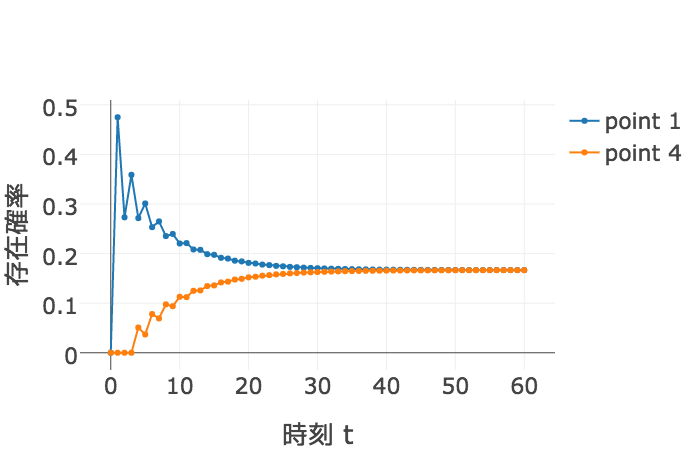
\includegraphics[width=\textwidth]{fig1.png}
  \caption{時刻 t における地点1,4でのバッタGの存在確率(s=0.05)}
\end{figure}

\begin{figure}
  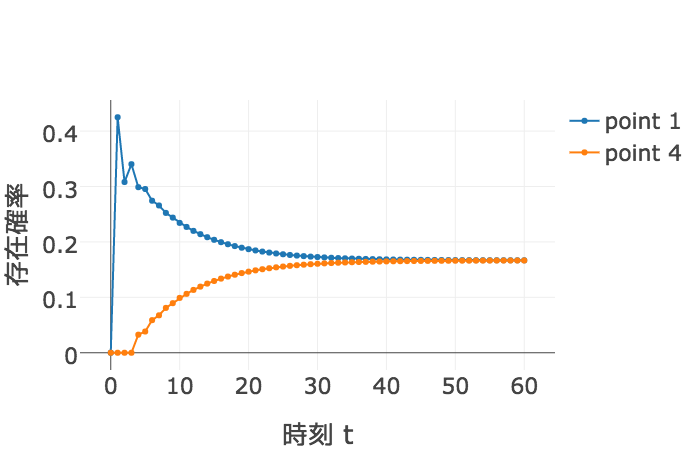
\includegraphics[width=\textwidth]{fig2.png}
  \caption{時刻 t における地点1,4でのバッタGの存在確率(s=0.15)}
\end{figure}

\begin{figure}
  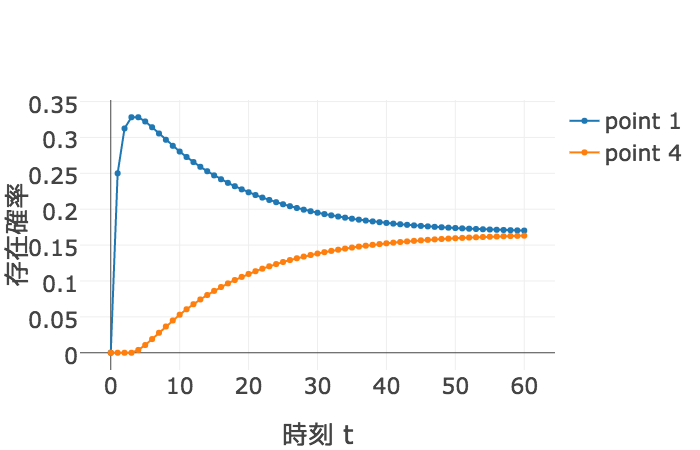
\includegraphics[width=\textwidth]{fig3.png}
  \caption{時刻 t における地点1,4でのバッタGの存在確率(s=0.5)}
\end{figure}

\subsection{パラメータcによるバッタGの振る舞いの変化}
	ソースコード3のプログラムを用いて、s=0.15とし、c=0.7,0.5,0.45の3つの場合について、前節と同様に、時刻$0 \leq t \leq 60$において各地点にGがいる確率を計算した。この結果を利用し、$t=60$において各地点にGがいる確率をグラフにしたのが、図4,5,6である。

\begin{figure}
  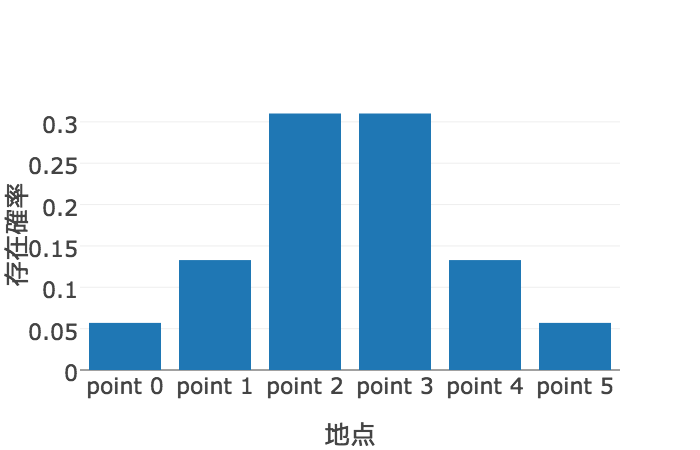
\includegraphics[width=\textwidth]{fig4.png}
  \caption{ t=60における各地点でのGの存在確率(c=0.7)}
\end{figure}

\begin{figure}
  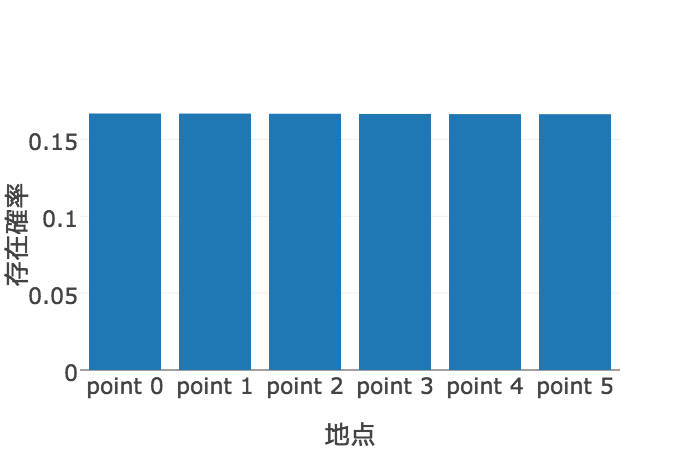
\includegraphics[width=\textwidth]{fig5.png}
  \caption{ t=60における各地点でのGの存在確率(c=0.5)}
\end{figure}

\begin{figure}
  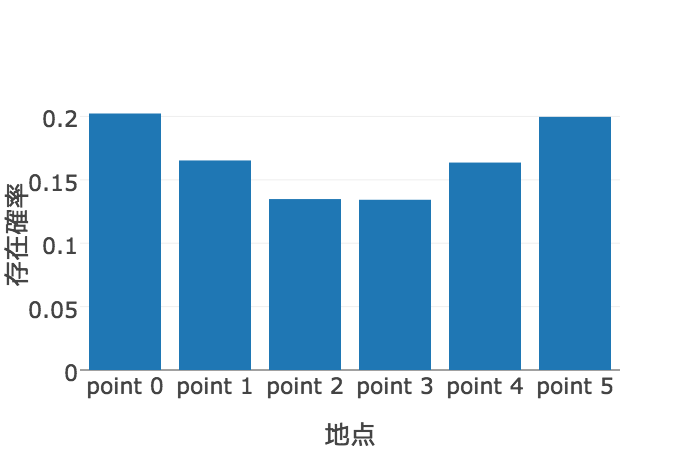
\includegraphics[width=\textwidth]{fig6.png}
  \caption{ t=60における各地点でのGの存在確率(c=0.45)}
\end{figure}

\subsection{ニュートン法による非線形方程式の解}

以下の2つの非線形方程式について、ソースコード4のプログラムを用いて、ニュートン法によって定められた範囲の解を求めた。

\begin{eqnarray}
	- 2.2 x^4 + 3.5x^3 + 4.1x^2 + 3.3x - 2.7 & = & 0, (0 \leq x \leq 1) \\
	- {\rm cos}(2x+2) + {\rm exp}(x+1) - 2x -30 & = & 0, (0 \leq x \leq \pi)
\end{eqnarray}

計算結果として、(1)に対しては$x = 0.4685126936655117$、(2)に対しては$x = 2.6107790395825665$という解が得られた。

\section{考察}

\subsection{行列とベクトルの演算を行う関数の実装}
\subsection{バッタGの移動}
\subsection{パラメータcによるバッタGの振る舞いの変化}
\subsection{ニュートン法による非線形方程式の解}

\end{document}